\documentclass{llncs}
%\usepackage{llncsdoc}
\usepackage{epsfig}
\usepackage{graphicx}

%\usepackage{caption}
%\usepackage{subcaption}

\newtheorem{mydef}{Def.}
\newtheorem{myhyp}{Hypothesis}

\usepackage{url}
\usepackage{hyperref}

\pagestyle{empty}

% PAKDD 2018: maximum 12 pages
% Abstract max 200 words
% title, abstract: 1/2 page
% introduction: 1 1/2 page (2 pages so far)
% related work: 1 to 1 1/2 pages (3 pages so far)
% method: 4 pages (7 pages so far)
% experiments: 3 (10 pages so far)
% discussion /conclusion: 1 page
% citations 1

% ====================================================================

% Eamonn ICDM'10 tutorial slides
% - clear problem statement in abstract
% - To convince a reviewer, you must think like a reviewer

% Writing the paper:
% - Make a working title
% - Introduce the topic and define (informally at this stage)
%   terminology
% - Motivation: Emphasize why is the topic important
% - Relate to current knowledge: what’s been done
% - Indicate the gap: what need’s to be done?
% - Formally pose research questions
% - Explain any necessary background material.
% - Introduce formal definitions.
% - Introduce your novel algorithm/representation/data structure etc.
% - Describe experimental set-up, explain what the experiments will
%   show
% - Describe the datasets
% - Summarize results with figures/tables
% - Discuss results
% - Explain conflicting results, unexpected findings and discrepancies
%   with other research
% - State limitations of the study
% - State importance of findings
% - Announce directions for further research
% - Acknowledgements
% - References
%
% - Don’t make the reviewer of your paper think!
% - Reviewers make an initial impression on the first page and don’t
%   change 80% of the time
% - A good introduction with a good motivation is half your success
% - By the end of the introduction the reviewer mustknow.
%   - What is the problem?
%   - Why is it interesting and important?
%   - Why is it hard?why do naive approaches fail?
%   - Why hasn't it been solved before?(Or, what's wrong with previous
%     proposed solutions?)
%   - What are the key components of my approach and results?Also
%     include any specific limitations.
%   - A final paragraph or subsection: “Summary of Contributions”.
%     It should list the major contributions in bullet form,
%     mentioning in which sections they can be found. This material
%     doubles as an outline of the rest of the paper, saving space and
%     eliminating redundancy
% - Unjustified Choices (are bad)
% - Optimal: Does not mean `very good'
% - Proved: Does not mean `demonstrated'
% - Significant: There is a danger of confusing the informal statement
%   and the statistical claim
% - Use all the Space Available
% - Avoid Weak Language: aim, attempt, might, etc.
% - Use the Active Voice
% - ALWAYS put some variance estimate on performance measures (do
%   everything 10 times and give me the variance of whatever you are
%   reporting)

% Figures:
% - Don't cover the data with the labels!
% - Color helps -Direct labeling helps -Meaningful captions help
%
% Common problem with figures:
% 1.Too many patterns on bars
% 2.Use of both different symbols and different lines
% 3.Too many shades of gray on bars
% 4.Lines too thin (or thick)
% 5.Use of three-dimensional bars for only two variables
% 6.Lettering too small and font difficult to read
% 7.Symbols too small or difficult to distinguish
% 8.Redundant title printed on graph
% 9.Use of gray symbols or lines
% 10.Key outside the graph
% 11.Unnecessary numbers in the axis
% 12.Multiple colors map to the same shade of gray
% 13.Unnecessary shading in background
% 14.Using bitmap graphics (instead of vector graphics)
% 15.General carelessness

% ====================================================================

% TODO:
% - clearly point out novelty of this work
% - contribution compared to earlier work

\begin{document}

% Peter 31 Oct: Current title does not really reflect the topic I
% think:
%\title{Exploring approaches to probabilistic record linkage using
%        similarity searching}
% Peter 31 Oct: What about
\title{Efficient and Effective Metric Space Indexing for Complete
       Record Linkage
       Al: Exploring approaches to probabilistic record linkage using similarity searching (metric space indexing?) }
%  \thanks{The authors would like to thank the ...|

\author{Submitted for double-blind review}
%\author{Özgür Akgün\inst{1} and Alan Dearle\inst{1} and Graham Kirby\inst{1} Peter Christen\inst{2}

%\institute{School of Computer Science,
%           University of St Andrews, \\
%           St Andrews, Scotland.~
%           Contact: \email{ozgur.akgun@st-andrews.ac.uk}

%\institute{Research School of Computer Science,
%           The Australian National University, \\
%           Canberra, Australia.~
%           Contact: \email{peter.christen@anu.edu.au}


\maketitle

% MAX 200 words
\begin{abstract}
Probabilistic record linkage is the process of identifying records that refer to
the same real-world entities across two or more databases in situations where entity identifiers are unavailable.
It requires  similarities between records to be approximated using common attributes (such as names, addresses, phone numbers) and for pairs of records to be classified as matches or non-matches.
Record linkage is usually performed in a two step process;  in the
first step a blocking or indexing is employed to efficiently group similar
candidate record pairs which are then compared in more detail and
classified in the second step.

As we show in this paper, even state-of-the-art blocking and
indexing techniques such as locality sensitive hashing, have two
major drawbacks. First, they often remove some true matching record
pairs that have high similarities due to their heuristic nature,
leading to a loss of recall. Second, they include many record pairs
with low similarity leading to high computational requirements.
Combined, this means a reduction of both effectiveness and efficiency.
% * <al@st-andrews.ac.uk> 2017-10-31T08:46:25.069Z:
%
% > efficiency
%
% ^.

We propose a metric indexing approach to \emph{complete} record
linkage, which ensures all record pairs that have a similarity above
a certain similarity threshold are being \textbf{compared}, while no pairs
with a similarity below the threshold are \textbf{compared}. Our approach
leads to a one-step record linkage process which combines indexing
with comparison and classification resulting in improved
effectiveness and efficiency as we experimentally evaluate on several
real-world databases.
Parameter space: good linkage bad linkage don't know which without ground truth. M Trees always high no config -> high confidence.

\end{abstract}

\keywords Entity resolution; data matching; similarity search;
         blocking.

% ====================================================================

\section{The Plan}

\vspace{5mm}

Plan in a bulleted list:

\begin{itemize}
\item Design: Traditionally it has two stages. A blocking method needs to be developed separately from a similarity method. With similarity search based record linkage, there is only one method, and that is the similarity method.
\item Efficiency: I am not convinced of this, but Peter thinks there may be efficiency benefits. The reasoning behind this is that with blocking-based methods we would have to calculate some sort of a similarity value first. This value will only be used for blocking, and later a similarity value between candidate pairs will need to be calculated again.
\item Completeness: Similarity search based methods will be complete (with respect to the given similarity method) whereas blocking based methods (including LSH) are likely to be incomplete (there will be high-similarity pairs which are not places in the same block)
\item Data sets
\begin{itemize}
\item Kilmarnock Birth-Death
\item Skye Birth-Death
\item CORA
\item North Carolina Voter Registration DB
\end{itemize}
\item The following is a list of all methods we thought we would have to compare.
\begin{itemize}
\item Similarity search (M-Tree, others?)
\item LSH-blocking
\item Traditional blocking (e.g. Region, Surname) - \textbf{why this? - this was done in the paper: A Comparison of Blocking Methods for Record Linkage}
\item MIFile
\item Sorted Neighbourhood blocking - \textbf{why this?}
\end{itemize}
\item Pairs-completeness and pairs-quality (w.r.t high similarity instead of true-link status). I will expand on this a bit more later.
\item Comparison (for blocking based methods)
		Precision/Recall/F1-Measure
\item Which similarity methods are metric?
\item Run time and memory usage comparisons
\item Theorem. Precision might get better or worse with similarity search based methods, but recall should never get worse.
\end{itemize}

Note: The rest of this paper should be regarded as a placeholder for now.

% --------------------------------------------------------------------

% 1 1/2 pages maximum!

\section{Introduction}
\label{sec-intro}

% Peter, 20171112:

Record linkage, also known as entity resolution, data matching and
duplicate detection~\cite{Chr12}, is the process of identifying and
matching records that refer to the same real-world entities within or
across databases. The entities to be linked are often people (such as 
patients in hospital or customers in business databases), but record
linkage can also be applied to link consumer products or bibliographic
records~\cite{Chr12}. Record linkage is commonly challenged by the
lack of unique entity identifiers (keys) in the databases to be linked,
which prevents the use of a database join. Instead, the linkage of
records requires the comparison of the attributes (or fields) that are
available in common in the databases to be linked. For databases that
contain information about individuals, these attributes include the
names, address, dates of birth, and so on, of individuals.

To overcome data quality issues such as typographical errors and
variations (which are common in name and address values~\cite{Chr12}),
approximate string comparison functions (such as edit distance, the
Jaro-Winkler comparator, or Jaccard similarity~\cite{Chr12}) are used
to compare pairs of records, leading to a vector of similarities (one
similarity per attribute/field compared) for each pair. These
similarity vectors are then used to classify the compared record
pairs into matches (where it is assumed both records in a pair
correspond to the same real-world entity) and non-matches (where the
records are assumed to correspond to two different entities). Various
classification methods have been employed in record
linkage~\cite{Chr12,Don15}, ranging from simple threshold based to
sophisticated clustering and supervised classification techniques, as
well as active learning approaches~\cite{Wan15}.

Besides the two challenges of a lack of unique entity identifiers and
data quality (which will affect linkage quality), record linkage is
also challenged by the increasing sizes of the databases to be
linked~\cite{Don15}. To prevent the full pair-wise comparison of all
possible record pairs (which is quadratic in the sizes of the
databases to be linked), blocking techniques (commonly known as
\emph{indexing}~\cite{Chr12b}) are used. The basic idea of these
techniques is to split the databases into smaller blocks in a
computationally efficient way such that records that likely correspond
to the same entity are inserted into the same block. Only records that
are in the same block are then compared with each other in more
details.

While indexing techniques facilitate the efficient linkage of very
large data-bases~\cite{Don15}, they generally achieve scalability at
the cost of loss in linkage quality, because potentially true matching
record pairs are removed in the indexing step, leading to a reduction
in recall of the final linkage result~\cite{Chr12}. A variety of
indexing techniques, as discussed in more detail in the following
section, have been proposed, ranging from simple phonetic based
blocking~\cite{Chr12} and sorting of the databases~\cite{Dra12} to
locality sensitive hashing based techniques~\cite{Kim10,Steorts2014}.
Unsupervised~\cite{Kej13,Ram15} and supervised~\cite{Bil06,Mic06} 
learning techniques of optimal blocking schemes have also been
proposed.

\begin{figure}[!t]
  \centering
  %\scalebox{1.0}[1.0]
  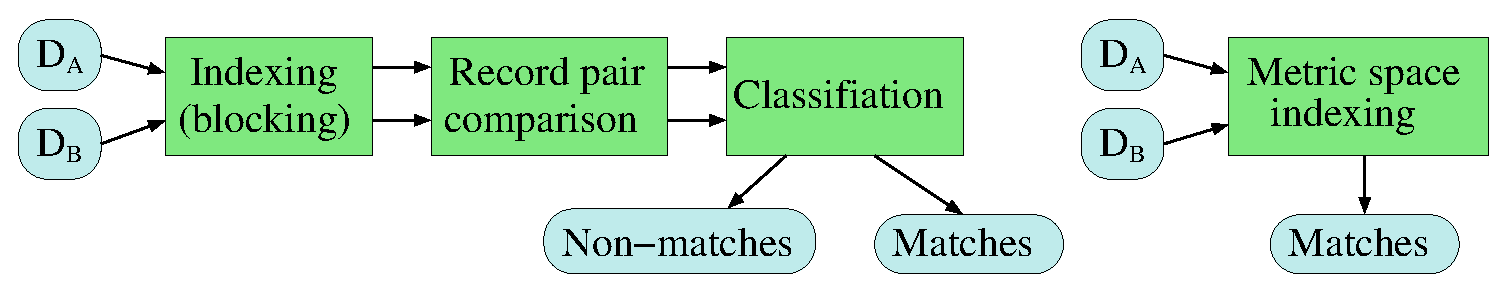
\includegraphics[width=1.0\textwidth]{figures/linkage-process}
  \caption{Overview of the steps of the traditional record linkage
           process (left-hand size) and our proposed metric space
           indexing approach (right-hand size), as described in
           Sect.~\ref{sec-intro}, where records from two databases,
           $\mathbf{D}_A$ and $\mathbf{D}_B$, are being linked.}
           \label{fig-rl-process}
\end{figure}

The overall process of a record linkage application, where indexing is
preformed prior to the comparison and classification steps, as
illustrated in Fig.~\ref{fig-rl-process}, adds a further practical
complexity. Indexing, comparison and classification are often conducted
using algorithms selected (and their parameters set) based on technical
and domain expertise of the user of the record linkage system, followed by a manual
assessment (auditing) of the linkage outcomes~\cite{Chr12}. If the quality of the
resulting links is not good enough for a certain application, the
linkage process needs to be repeated with different parameter settings
and possibly also alternative algorithms selected. This can result in
a time-consuming and labor intensive iterative process. A major
challenge is often the heuristic nature of indexing, where the choice
of a certain indexing technique and its parameters (including which
attributes to use in indexing) will determine the final outcome of a
linkage.
% Repeat:
% If a certain blocking approach results in a loss of recall in the
%final linkage results, the blocking needs to be redone, an often time
%consuming process.

In this paper we explore how existing indexing techniques can lead to
loss in recall, even for record pairs that are highly similar and
likely correspond to true matches. As a result, using such techniques
can lead to \emph{incomplete} record linkage results. To overcome this
problem, we advocate the use of \emph{metric space indexing} (MSI)
approaches, where it is possible to guarantee that all record pairs,
up-to a certain distance threshold, are included in the record linkage
results. MSI also prevents the expensive detailed comparison of record
pairs that have low similarities but that need to be compared because
they have been inserted into the same block with traditional indexing
techniques. Furthermore, MSI allows the combination of the indexing,
comparison and classification steps (as traditionally conducted
independently) into one single step, as shown in
Fig.~\ref{fig-rl-process}, making the overall record linkage process
both more efficient and more effective.

% Al: but is it? be careful of last sentence in final version.

% Peter 20171112: do we also need to mention we do not waste
% comparisons of record pairs with low similarities (i.e. those with
% a distance > max_dist)?

~ \\
\emph{Peter 20171111: here we need the figure showing that traditional
blocking techniques result in incomplete record linkage, while metric
indexing does not.}
~ \\

While MSI has been used extensively in areas such as database indexing
and general nearest neighbor search, its use in record linkage so far
has been limited. 
% Al - So take it out - I recently found and cited a paper that uses R trees later in the paper?

% Peter 20171112: a pretty dangerous statement. if wrong we're stuffed.. 
% but I am not really aware of MSI approaches in RL..
Many different MSI approaches have been developed, such as various
metric tree structures~\cite{}. 
% Peter 20171112: needs same text from you guys on MSI..
In this paper, we will use the MSI techniques of M-tree and M-file (?)
and show how their use can facilitate an improvement of both
efficiency and effectiveness of the record linkage process.

~ \\
\emph{
to add: something about similarity spaces / metric spaces, M-trees and its
more recent advanced/improved versions, and how they have been used in
similarity search.}

\emph{to add: How our work is different from these other metric space works, and
description of our contributions.
}
~ \\

\smallskip
\textbf{Contributions:} We make three specific contributions in this
paper: (1) We investigate how existing indexing techniques can result
in \emph{incomplete} record linkage results, as well as in an
in-efficient record linkage process. (2) We explore MSI for record
linkage and propose a MSI based linkage approach that achieves
\emph{complete}, efficient and effective record linkage. (3) We
evaluate our approach on several real-world data sets from diverse
domains and show its advantages over existing indexing techniques for
record linkage.

% old stuff below



\iffalse  % *******************************************************
% we can't write this as it reveals us in the double-blind review
% we could ad to final paper
The motivation for this work is the Digitising Scotland project (Dibben 2012), which is in the process of transcribing and linking all the vital events recorded in Scotland between 1856 and 1977. This data set will, when complete, include around 14 million birth records, 11 million death records and 4 million marriage records. As part of the work, certain data fields (locations, occupations and causes of death) are also being classified to the relevant standard coding schemes.
\fi  % *********************************************************

% --------------------------------------------------------------------

% 1 page maximum!

\section{Related Work}
\label{sec-related}

We now briefly review relevant related work in the areas of indexing
for record linkage (for a recent survey see~\cite{Chr12b,Pap16}),
and metric space indexing~\cite{Zezula2010}.

\smallskip
\textbf{Indexing for Record Linkage:}
Techniques to link records across databases have been developed for
over five decades~\cite{Fel69,New59}, and the scalability of linking
has been an ongoing challenge as databases are continue to grow in
size and complexity. Traditional blocking~\cite{Chr12b} use a single
or a combination of attributes (known as a \emph{blocking key}) to
insert records that have the same value(s) in a blocking key into
the same block. Only records within the same block are then combined
with each other. To overcome variations and misspellings, the values
used in blocking keys can be phonetically encoded using functions
such as Soundex, NYSIIS, or Double-Metaphone~\cite{Chr12}. These
techniques convert a string (assumed to be a name) into a code
according to its pronunciation, assigning the same code to similar
sounding names (such as `Gail' and `Gayle').

A different approach to indexing is the sorted neighborhood 
method~\cite{Mon96}, where the databases to be linked are sorted
according to a \emph{sorting key} (usually a concatenation of the
values from several attributes). A sliding window is then moved over
the databases and only records within the same window are being
compared. Techniques that adaptively shrink or expand the window size based on
the characteristics of the sorting key values have shown to improve
both linkage efficiency and quality~\cite{Dra12}.

% should we mention canopy clustering? best to only briefly mention
% techniques we do not use in our comparison

Locality sensitive hashing (LSH), as originally proposed to allow
efficient nearest-neighbor search in high-dimensional
spaces~\cite{Ind98}, has been employed in record linkage as a blocking
technique where attribute values are hashed multiple times, and
blocks are created from those records that share some hash values.
\emph{HARRA} is a record linkage approach based on Min-hash and LSH
which blocks, compares, and then merges linked records in an iterative
fashion, where merged records are re-hashed to improve overall linkage
quality. Steorts et al.~\cite{Steorts2014} recently evaluated two LSH
variations, with their main conclusion being that in order to get good
results LSH methods must be tuned to the particular databases being
linked. This requires good quality ground truth data which may be
unavailable or very expensive to obtain.

Existing blocking techniques have the drawbacks that they are
heuristics and commonly require domain knowledge, such as the choice
of blocking or sorting key used. Errors and variations in the
attributes used for blocking also result in records being inserted
into a wrong block and thus true matches being missed. As a result,
existing blocking techniques can lead to \emph{incomplete} linkage,
and that many of the record pairs compared in a block turn out to be
pairs with low similarities that correspond to non-matches, resulting
in \emph{inefficient} linkage.

% Peter until here, 20171113 ************

\iffalse

% commented, as overall related works should be around 1 page max

Steorts et al. \cite{Steorts2014} examined various approaches to blocking records raging from traditional blocking to variations on Locality Sensitive Hashing (LSH). They assert that traditional blocking based on human selected fields has two major drawbacks. The first is that the blocks that are formed are so large that it remains computationally impractical to compare all the records in the block. Secondly, since similarity is based on a subset of the available fields, records in the same block may differ greatly in the fields that are not considered. \textbf{{this is true of our technique - explore somewhere}}. The paper examines two LSH variations - transitive LSH {ref needed} (TLSH) and K-Means LSH (KLSH). {\textbf{describe these where?}} 
Using simulated data based on people, their data of birth and postal address to evaluate the efficacy of these approaches, they demonstrate that KLSH performs as well or better than commonly used approaches to blocking such as those described \textbf{above}. However, they point out that, like all LSH methods, in order to get good results, it must be tuned to the particular dataset being linked. This in turn requires good ground truth about the dataset which may be unavailable, impossible or very expensive to obtain. \textbf{We examine and address these problems in this paper.}

\fi

% - - - - - - - - - - - - - - - - - - - - - - - - - - - - - - - - - - -

\smallskip
\textbf{Metric Space Indexing:}


% Al's writing below

In \cite{Yu2016} Yu et al. have written an extensive survey on string similarity and join in which the problem is defined as "Given two sets of objects, similarity join aims to find all similar pairs from the two collections". Part of the survey is concerned the  algorithms used to compare two records which are characterised as being character-based, token-based or hybrid. The first, which includes approaches such as Levenshtein {ref needed} use character differences in the strings being compared, the second, which includes techniques such as Jaccard similarity {ref needed}, treats the records as sets of tokens and utilises set similarity, the third hybridises the two approaches. Yu's divides join algorithms (which unify records - also known as linkage) into three categories: a number of techniques based on filtering, verification based and threshold-based. Filtering involves generating signatures for each record and creating inverted lists containing records with common signatures and pruning records with no common signatures. Verification algorithms involve calculating the exact distances of a prefix of the data, and using another technique to estimate the edit distance between records. If the estimated distance is larger than the desired similarity threshold, the candidate may be discarded. The last category (threshold based) includes M-tree, Trie-Join, Pass-Join and Partenum. These approaches all require indexing structures to be constructed that are then used to support comparison.  

{\textbf{do we need to describe these?}}

 \cite{Li2006} describes a method of performing linkage using R-trees {ref needed} that fall into the threshold based category of Yu et al. Their approach demonstrates that high precision and recall may be achieved by measuring Jaccard similarity over selected fields from the records being compared. In their evaluation , their approach achieved a recall of 99 percent in experiments in which conjunctions of similarities over fields were used. In a later paper \cite{Ciaccia97indexingmetric}  Ciaccia et al. demonstrate that using M-trees are almost always more efficient than R-trees.

summarise related work in metric spaces as used in record linkage

other related works as relevant

% end of related work should be around end of page 3!

% --------------------------------------------------------------------

% do we need a section on preliminaries, notation, etc?
% ideally techniques are described formally, possibly via pseudo-code
% algorithmic descriptions

\section{Approach}
\label{sec-approach}

In this paper we explore the efficacy of the use of different similarity search algorithms in probabilistic record linkage. We explore two inexact algorithms: LSH-minhash and MIFile \cite{amato2014mi} one exact method: mTrees \cite{paolociaccia2m}. We also use a simple brute force (nested-loop) exact technique as a baseline for comparison although this approach can only be applied to the smallest of our datasets. All of our experiments have a number of configuration parameters with which we can configure the search space and algorithm behaviours. All have a \textit{distance threshold} below which two records are deemed to represent a link.

In the brute force approach two nested loops are used to compare every record with every other non identical record. The complexity of this approach is n2. If a link can be found with whatever distance metric is used, this approach will find it. Each of our datasets contains ground truth with which we can establish the records that are true links and those that are not. 

The LSH-minhash approach is a fast but inexact method of performing similarity search. It has a number of tuning parameters: \textit{shingle\_size}, the \textit{number\_of\_bands} and the \textit{band\_size}. These are explained in the following algorithm description which follows a standard LSH approach. Firstly all the fields of the record are turned into strings and concatenated. Next the strings are \textit{shingled} into a set of n-grams according to the \textit{shingle\_size} parameter. Next a set of randomly, deterministically generated hash functions are applied to each of the sets of n-grams and the smallest (the minhash) of each application is added to a signature. The number of hashes used and thus the size of the signature is determined by the product of the {number\_of\_bands} and the {band\_size}.  Lastly the signature is divided into {number\_of\_bands} segments and the elements from the band are hashed again to create a number of keys. The original record is added to a hashmap associated with each of the keys. It can be shown that the similarities between signatures generated in the second step have very close Jaccard similarity to the original string and that if an arbitrary record is run through this process the records found in the map are close to the record being searched with good precision and recall. We will further explore these properties in this paper. To perform a {\textit{nearest-neighbour}} lookup, the query value is hashed using the procedure described above and the union of set of of values found for all hashes in the hashmap are returned. If desired, these may then be filtered by performing distance calculations on the results.

The MIFile \cite{amato2014mi} approach is inexact technique for performing similarity search based on metric spaces. Using  MI\_file,  each record is represented by the ordering of distances from a collection of reference objects. It is based on the idea that two records close to each other will have similar neighbours and will thus be represented by similar of distances from the chosen reference objects. 
In order to create the indexes, for each value to be added to the data-structure, first the k nearest reference objects (governed by a fixed parameter) are found, each is given a score (drawn from 1,2,3... based on the reference object's position from the value). Next for each score, a  mapping is created in an inverted index mapping from the value to the score of each reference object and a representation of the data associated with the reference object and the value inserted.  In order to perform a \textit{nearest-neighbour} lookup, first the k nearest reference objects (bounded by a second fixed parameter). Next the objects closest to these reference objects are extracted from the inverted map by choosing the neighbours with the highest score. Much of the search space may be eliminated by  keeping track of the scores that  can contribute to the nearest neighbours.

M-trees support exact search operations over a set of values over a metric space (distances must support  triangle inequality - distance(i,j) + distance(j,k ) >= distance(i,k)). In addition to supporting exact search the operations supported by M-trees are richer than the other data structures described above and include \textit{range search} (all values within distance d and some query q), \textit{nearest-neighbour} (the closest value to q), and \textit{nearestN} (the N closest n objects to q). An M-tree is a balanced tree structure comprised of fixed sized nodes that can each store up to \textit{M} children. In addition to the children, each node contains a reference to an object being indexed, a pointer and the distance to its parent, and a radius (described below). The radius of an internal node called a \textit{routing-node} represents the  furthest distance to any of its children. Thus all the children may be visualised as being contained within a ball of radius \textit{r} from the parent. M-trees are grown from the roots upward and require dynamic tree rebalancing when set of children become full (of size \textit{M}).

% TODO coverage: proportion of all rec pairs with a certain similarity (independent of their match status) that are being generated by a blocking  technique - what does above refer to? al

% - - - - - - - - - - - - - - - - - - - - - - - - - - - - - - - - - -

% subsection

%  - - - - - - - - - - - - - - - - - - - - - - - - - - - - - - - - - -

%\subsection

% --------------------------------------------------------------------



%  - - - - - - - - - - - - - - - - - - - - - - - - - - - - - - - - - -

\subsection{Analysis and Limitations}
\label{sec-analysis}

maybe a complexity analysis? maybe an analysis of expected 
linkage quality?

% --------------------------------------------------------------------

\section{Experiments and Results}
\label{sec-expt}

We now describe the data sets we use in our evaluation and the
experimental setup we employed to evaluate our proposed metric
indexing approach.


% - - - - - - - - - - - - - - - - - - - - - - - - - - - - - - - - - -

% Peter 31 Oct: table style follows LNCS style guide

\begin{table}[t]
\caption{Characteristics of data sets used in experiments.
  \emph{Peter, 31 Oct: what else should we show here?}}
 \label{table-datasets}
  \centering
  \begin{scriptsize}
  %\addtolength{\tabcolsep}{-0.5pt}
  \begin{tabular}{ccccc}
  \hline\noalign{\smallskip}
  Data set~ & ~Number of~ & ~Number of true~
   & Attributes used? & ~?? \\
  name(s)  & records   & matching pairs &
    for indexing & ?? \\
  \noalign{\smallskip}
  \hline
  \noalign{\smallskip}
  NCVR  & ~224,073 / 224,061~ & ~148,036~ & ? & ? \\
  CORA  & 1,295             & title, authors, venue, year ? & ?
    & ? \\
  Isle of Skye & ? & ?
    & ? & ? \\
  Kilmarnock  & ? & ? & ? & ? \\
  \hline
  \end{tabular}
  \end{scriptsize}
\end{table}

% Peter, 31 Oct: To save space, don't use sub-sections but simply
% \textbf{}, such as:
% \smallskip
%\textbf{Data sets}:~

\subsection{Data Sets and Experimental Setup}
\label{sec-data}

We used four real data sets from three domains in our experiments. The
first is the CORA data set~\footnote{Available from:
\texttt{http://secondstring.sourceforge.net}}, which contains 1,295
(?) records that refer to XX machine learning publications.

The second are a pair of data sets based on the North Carolina Voter
Registration (NCVR) data sets\footnote{Available from: \texttt{http://dl.ncsbe.gov/}}, which we collected in June 2014 and
October 2016. Each of these two data sets contain over five million
records of voters and include attributes with their first names,
surnames, and addresses. Ground truth is provided via a \emph{NCID}
identifier which uniquely identifies a voter. In our experiments we
use two randomly selected sub-set of $224,073$ and $224,061$ records,
respectively, where $148,036$ of those refer to voters that occurred
in both original NCVR data sets but had name and/or address changes
over time (thus leading to around $66\%$ matching records).

% Peter, 31 Oct: can the following be shortened to 1 paragraph - tick - al.

We also experiment over two datasets prepared by researchers pursuing previous projects \cite{reid2002} and \cite{reid2006}, which act as pseudo subsets for the demographic linkage on which our work is primarily focused . One data set contains records of vital events registered on the Isle of Skye, a rural district, while the other contains records from Kilmarnock, an industrial town. Both cover the period 1861-1901. These are different types of communities, with different family structures and name distributions \cite{reid2002}. Both datasets are encoded with the same schemata and include names, sex, addresses and the names of each person's father and mother. Ground truth is provided using demographer encoded identifiers which provide (incomplete) linkage between the records.  The Isle of Skye dataset comprises around 17,600 birth records, 12,300 death records, and 2,700 marriage records. Relating to the experiments described below, this dataset contains 2,900 links from a birth record to the child's death record. The Kilmarnock data set contains around 38,400 birth records, 23,700 death records, and 8,700 marriage records with a similar schema to the Skye data. In this dataset demographers identified  2,900 links from a birth record to the child's death record.

% --------------------------------------------------------------------

\section{Conclusions and Future Work}
\label{sec-concl}

% --------------------------------------------------------------------

\bibliographystyle{abbrv}
\bibliography{paper.bib} 



\end{document}

% ====================================================================
